\documentclass{article}
\usepackage{tikz}
\usetikzlibrary{decorations.pathreplacing}
\usepackage{xcolor}
\usepackage[margin=1in]{geometry}

\begin{document}

\begin{figure}
\centering
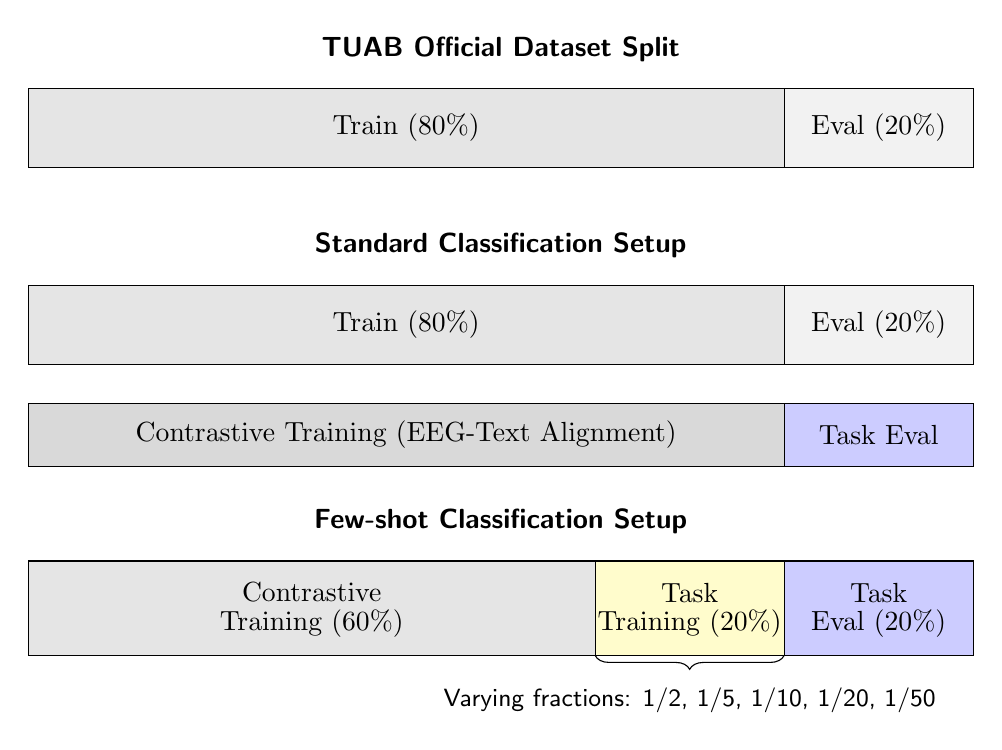
\begin{tikzpicture}[
    box/.style={rectangle, draw, minimum height=0.8cm, font=\sffamily},
    section/.style={font=\sffamily\bfseries}
]
    % Title
    % \node[section] at (6,0.5) {Data Partitioning Strategy};
    
    % TUAB Official Split
    \node[section] at (6,-0.5) {TUAB Official Dataset Split};
    
    \draw[fill=gray!10, draw=black] (0,-1) rectangle (12,-2);
    \draw[fill=gray!20, draw=black] (0,-1) rectangle (9.6,-2);
    
    \node at (4.8,-1.5) {Train (80\%)};
    \node at (10.8,-1.5) {Eval (20\%)};
    
    % Standard Classification
    \node[section] at (6,-3) {Standard Classification Setup};
    
    \draw[fill=gray!10, draw=black] (0,-3.5) rectangle (12,-4.5);
    \draw[fill=gray!20, draw=black] (0,-3.5) rectangle (9.6,-4.5);
    
    \node at (4.8,-4) {Train (80\%)};
    \node at (10.8,-4) {Eval (20\%)};
    
    \draw[fill=gray!30, draw=black] (0,-5) rectangle (9.6,-5.8);
    \draw[fill=blue!20, draw=black] (9.6,-5) rectangle (12,-5.8);
    
    \node at (4.8,-5.4) {Contrastive Training (EEG-Text Alignment)};
    \node at (10.8,-5.4) {Task Eval};
    
    % Few-shot Classification
    \node[section] at (6,-6.5) {Few-shot Classification Setup};
    
    \draw[fill=gray!10, draw=black] (0,-7) rectangle (12,-8.2);
    \draw[fill=gray!20, draw=black] (0,-7) rectangle (7.2,-8.2);
    \draw[fill=yellow!20, draw=black] (7.2,-7) rectangle (9.6,-8.2);
    \draw[fill=blue!20, draw=black] (9.6,-7) rectangle (12,-8.2);
    
    \node at (3.6,-7.4) {Contrastive};
    \node at (3.6,-7.8) {Training (60\%)};
    
    \node at (8.4,-7.4) {Task};
    \node at (8.4,-7.8) {Training (20\%)};
    
    \node at (10.8,-7.4) {Task};
    \node at (10.8,-7.8) {Eval (20\%)};
    
    % Add underbrace for the Task Training box
    \draw [decorate,decoration={brace,amplitude=5pt,mirror}] (7.2,-8.2) -- (9.6,-8.2) 
      node[midway,below=8pt,font=\sffamily\small] {Varying fractions: 1/2, 1/5, 1/10, 1/20, 1/50};
    
\end{tikzpicture}
\caption{Experimental data partitioning strategies for EEG-CLIP. The top section shows the official TUAB dataset split. The middle section illustrates the standard classification setup where the training portion is used for contrastive learning between EEG signals and text descriptions. The bottom section visualizes the few-shot learning approach with varying fractions of the labeled training data.}
\label{fig:data-partition}
\end{figure}

\end{document}